This is the first sub section that user interacts with. When the user opens the mobile application for the first time details for SignUp is displayed. Then the user enters all the information required for SignUp including all the valid user name and password to create a account. Then an account for the user is created.

\subsection{UI Controller}


\begin{figure}[h!]
	\centering
 	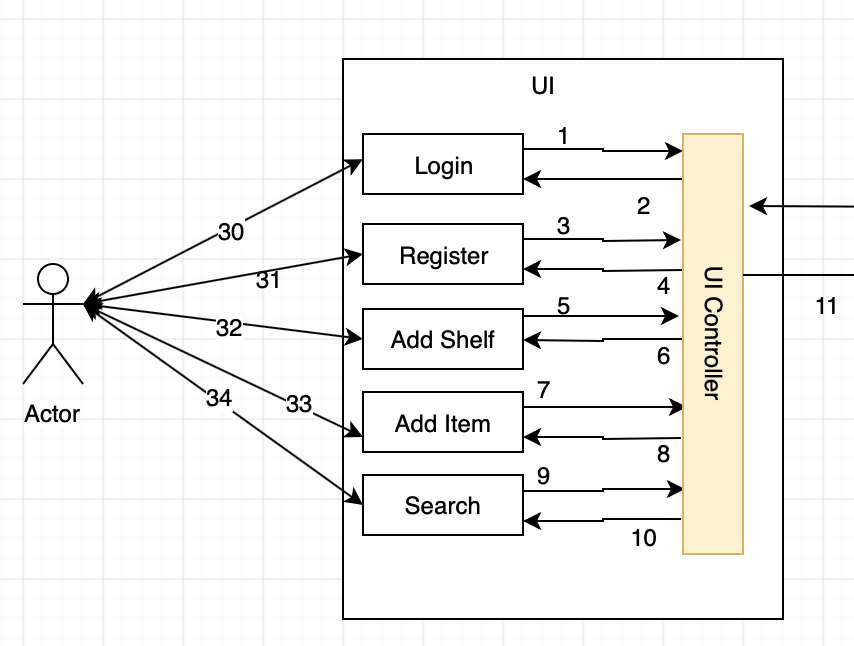
\includegraphics[width=0.60\textwidth]{images/uicontroller}
 \caption{Example subsystem description diagram}
\end{figure}

\subsubsection{Assumptions}
Following assumptions are made for this SubSystem:
\begin{itemize}
    \item 
\end{itemize}

\subsubsection{Responsibilities}
Following are the responsibilities of this SubSystem:
\begin{itemize}
    \item 
\end{itemize}

\subsubsection{Subsystem Interfaces}
Each of the inputs and outputs for the subsystem are defined here. Create a table with an entry for each labelled interface that connects to this subsystem. For each entry, describe any incoming and outgoing data elements will pass through this interface.

\begin {table}[H]
\caption {Subsystem interfaces} 
\begin{center}
    \begin{tabular}{ | p{1cm} | p{6cm} | p{3cm} | p{3cm} |}
    \hline
    ID & Description & Inputs & Outputs \\ \hline
    \#xx & Description of the interface/bus & \pbox{3cm}{input 1 \\ input 2} & \pbox{3cm}{output 1}  \\ \hline
    \#xx & Description of the interface/bus & \pbox{3cm}{N/A} & \pbox{3cm}{output 1}  \\ \hline
    \end{tabular}
\end{center}
\end{table}

\subsection{Login}


\begin{figure}[h!]
	\centering
 	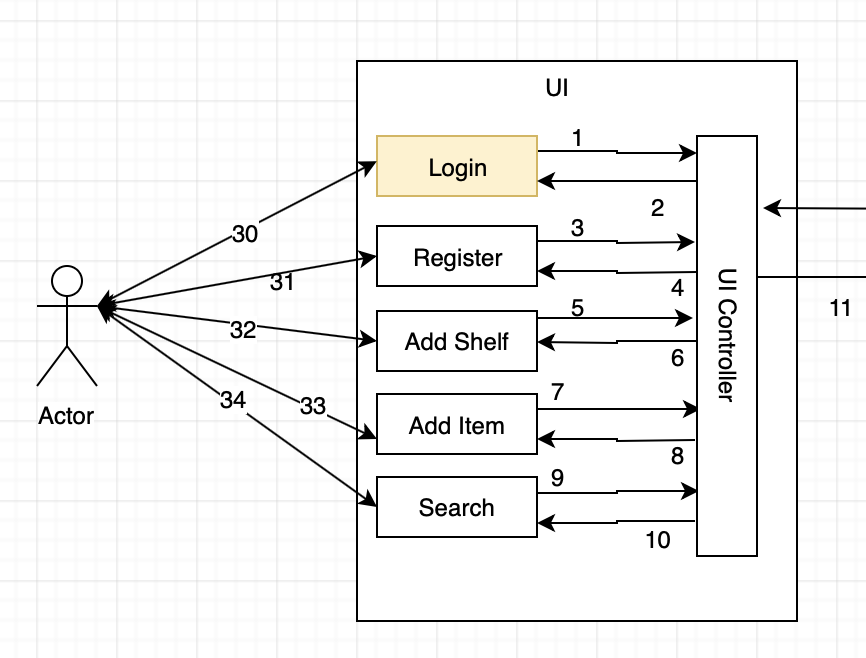
\includegraphics[width=0.60\textwidth]{images/login}
 \caption{Example subsystem description diagram}
\end{figure}

\subsubsection{Assumptions}
Following assumptions are made about this SubSystem:
\begin{itemize}
    \item 
\end{itemize}

\subsubsection{Responsibilities}
These are the following responsibilities of this subsystem:
\begin{itemize}
    \item 
\end{itemize}

\subsubsection{Subsystem Interfaces}
Each of the inputs and outputs for the subsystem are defined here. Create a table with an entry for each labelled interface that connects to this subsystem. For each entry, describe any incoming and outgoing data elements will pass through this interface.

\begin {table}[H]
\caption {Subsystem interfaces} 
\begin{center}
    \begin{tabular}{ | p{1cm} | p{6cm} | p{3cm} | p{3cm} |}
    \hline
    ID & Description & Inputs & Outputs \\ \hline
    \#xx & Description of the interface/bus & \pbox{3cm}{input 1 \\ input 2} & \pbox{3cm}{output 1}  \\ \hline
    \#xx & Description of the interface/bus & \pbox{3cm}{N/A} & \pbox{3cm}{output 1}  \\ \hline
    \end{tabular}
\end{center}
\end{table}

\subsection{Register}


\begin{figure}[h!]
	\centering
 	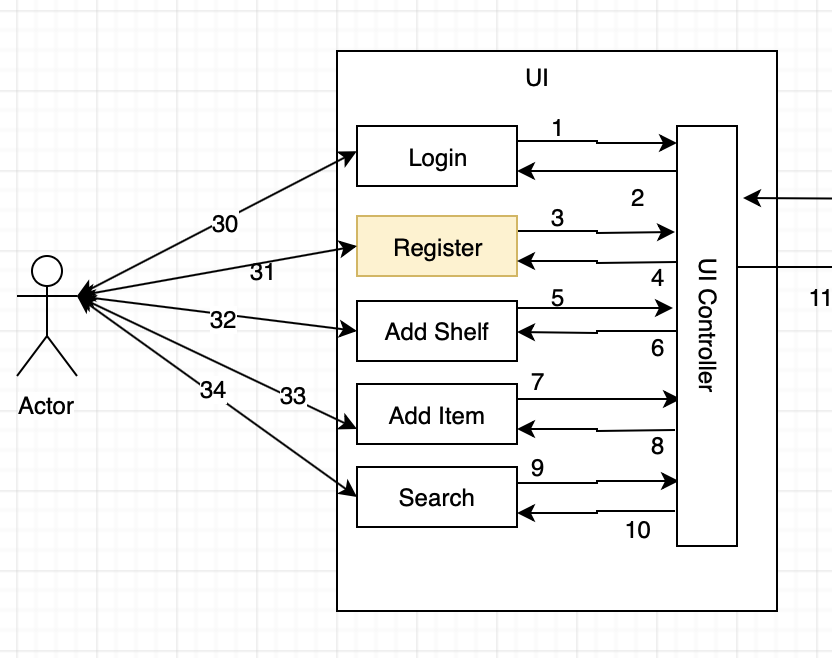
\includegraphics[width=0.60\textwidth]{images/register}
 \caption{Example subsystem description diagram}
\end{figure}

\subsubsection{Assumptions}
Following are the assumption of SubSection Email/Password Validation:
\begin{itemize}
    \item
\end{itemize}
\subsubsection{Responsibilities}
Following responsibilities must be carried out by this SubSystem:
\begin{itemize}
    \item
\end{itemize}

\subsubsection{Subsystem Interfaces}
Each of the inputs and outputs for the subsystem are defined here. Create a table with an entry for each labelled interface that connects to this subsystem. For each entry, describe any incoming and outgoing data elements will pass through this interface.

\begin {table}[H]
\caption {Subsystem interfaces} 
\begin{center}
    \begin{tabular}{ | p{1cm} | p{6cm} | p{3cm} | p{3cm} |}
    \hline
    ID & Description & Inputs & Outputs \\ \hline
    \#xx & Description of the interface/bus & \pbox{3cm}{input 1 \\ input 2} & \pbox{3cm}{output 1}  \\ \hline
    \#xx & Description of the interface/bus & \pbox{3cm}{N/A} & \pbox{3cm}{output 1}  \\ \hline
    \end{tabular}
\end{center}
\end{table}


\subsection{Add Self}


\begin{figure}[h!]
	\centering
 	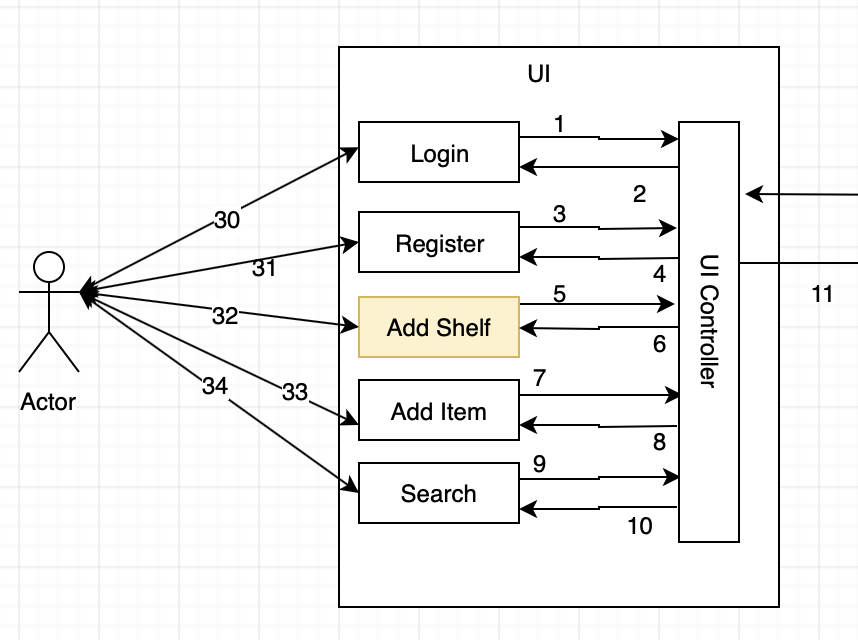
\includegraphics[width=0.60\textwidth]{images/addshelf}
 \caption{Example subsystem description diagram}
\end{figure}

\subsubsection{Assumptions}
Following assumptions are made about this SubSystem:
\begin{itemize}
    \item 
\end{itemize}

\subsubsection{Responsibilities}
These are the following responsibilities of this subsystem:
\begin{itemize}
    \item 
\end{itemize}

\subsubsection{Subsystem Interfaces}
Each of the inputs and outputs for the subsystem are defined here. Create a table with an entry for each labelled interface that connects to this subsystem. For each entry, describe any incoming and outgoing data elements will pass through this interface.

\begin {table}[H]
\caption {Subsystem interfaces} 
\begin{center}
    \begin{tabular}{ | p{1cm} | p{6cm} | p{3cm} | p{3cm} |}
    \hline
    ID & Description & Inputs & Outputs \\ \hline
    \#xx & Description of the interface/bus & \pbox{3cm}{input 1 \\ input 2} & \pbox{3cm}{output 1}  \\ \hline
    \#xx & Description of the interface/bus & \pbox{3cm}{N/A} & \pbox{3cm}{output 1}  \\ \hline
    \end{tabular}
\end{center}
\end{table}

\subsection{Add Item}
Add Item allows the user to add the items with the description of its different attributes. Attributes like name of product, brand name, manufacture date, best by date and size of product.


\begin{figure}[h!]
	\centering
 	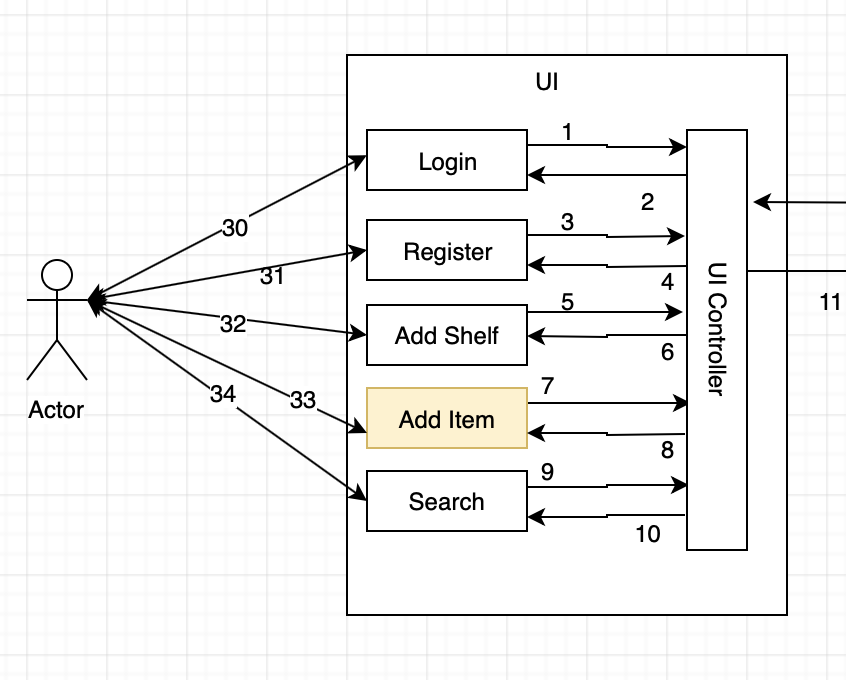
\includegraphics[width=0.60\textwidth]{images/additem}
 \caption{Example subsystem description diagram}
\end{figure}

\subsubsection{Assumptions}
Following assumptions are made about this SubSystem:
\begin{itemize}
    \item 
\end{itemize}

\subsubsection{Responsibilities}
These are the following responsibilities of this subsystem:
\begin{itemize}
    \item 
\end{itemize}

\subsubsection{Subsystem Interfaces}
Each of the inputs and outputs for the subsystem are defined here. Create a table with an entry for each labelled interface that connects to this subsystem. For each entry, describe any incoming and outgoing data elements will pass through this interface.

\begin {table}[H]
\caption {Subsystem interfaces} 
\begin{center}
    \begin{tabular}{ | p{1cm} | p{6cm} | p{3cm} | p{3cm} |}
    \hline
    ID & Description & Inputs & Outputs \\ \hline
    \#xx & Description of the interface/bus & \pbox{3cm}{input 1 \\ input 2} & \pbox{3cm}{output 1}  \\ \hline
    \#xx & Description of the interface/bus & \pbox{3cm}{N/A} & \pbox{3cm}{output 1}  \\ \hline
    \end{tabular}
\end{center}
\end{table}

\subsection{Search}


\begin{figure}[h!]
	\centering
 	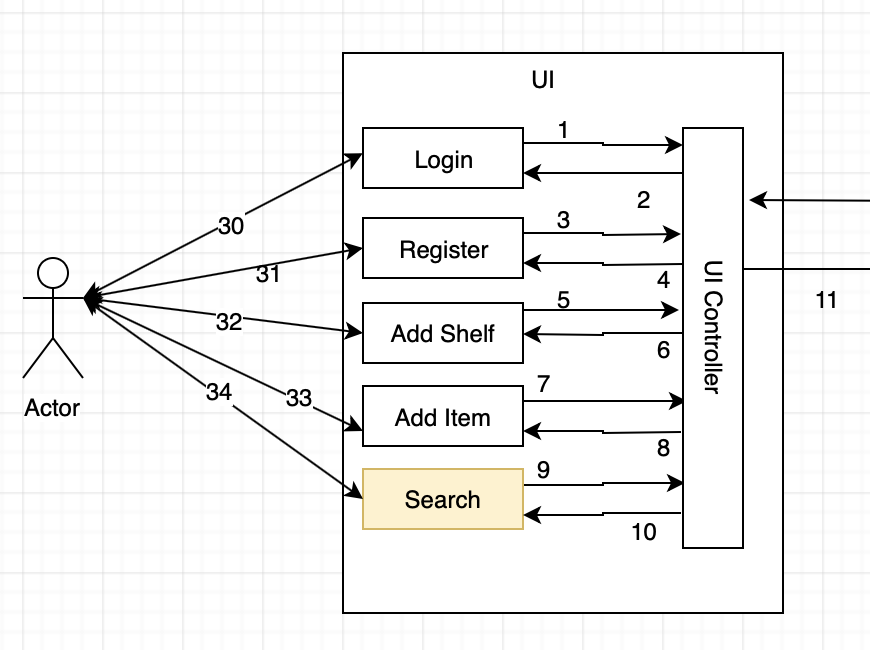
\includegraphics[width=0.60\textwidth]{images/search}
 \caption{Example subsystem description diagram}
\end{figure}

\subsubsection{Assumptions}
Following assumptions are made about this SubSystem:
\begin{itemize}
    \item 
\end{itemize}

\subsubsection{Responsibilities}
These are the following responsibilities of this subsystem:
\begin{itemize}
    \item 
\end{itemize}

\subsubsection{Subsystem Interfaces}
Each of the inputs and outputs for the subsystem are defined here. Create a table with an entry for each labelled interface that connects to this subsystem. For each entry, describe any incoming and outgoing data elements will pass through this interface.

\begin {table}[H]
\caption {Subsystem interfaces} 
\begin{center}
    \begin{tabular}{ | p{1cm} | p{6cm} | p{3cm} | p{3cm} |}
    \hline
    ID & Description & Inputs & Outputs \\ \hline
    \#xx & Description of the interface/bus & \pbox{3cm}{input 1 \\ input 2} & \pbox{3cm}{output 1}  \\ \hline
    \#xx & Description of the interface/bus & \pbox{3cm}{N/A} & \pbox{3cm}{output 1}  \\ \hline
    \end{tabular}
\end{center}
\end{table}

